\documentclass[tikz,border=0pt]{standalone}
\usepackage{xcolor}
\usetikzlibrary{calc}
% Palette: Sam_Comm_final.png by eye, each course's own, and data/frogs.json.
\definecolor{ink}{HTML}{3B2340}
\definecolor{sky}{HTML}{EFC46A}
\definecolor{skyhi}{HTML}{F5DA92}
\definecolor{skylow}{HTML}{E9B060}
\definecolor{cloud}{HTML}{F2D58A}
\definecolor{paper}{HTML}{FBEFD0}
\definecolor{cream}{HTML}{FFF6E0}
\definecolor{white}{HTML}{FFFFFF}
\definecolor{wallA}{HTML}{E88A73}
\definecolor{wallB}{HTML}{EE9F7E}
\definecolor{wallC}{HTML}{E47A7E}
\definecolor{wallD}{HTML}{F0B07E}
\definecolor{wallE}{HTML}{D9765F}
\definecolor{wallF}{HTML}{E99A8A}
\definecolor{greenA}{HTML}{8DBB7E}
\definecolor{greenB}{HTML}{6FA77A}
\definecolor{greenC}{HTML}{A9C97F}
\definecolor{greenD}{HTML}{5E9C6A}
\definecolor{greenE}{HTML}{4A8060}
\definecolor{meadow}{HTML}{B5CF86}
\definecolor{meadowdark}{HTML}{9DBE74}
\definecolor{window}{HTML}{F6E7A0}
\definecolor{windark}{HTML}{8C5A64}
\definecolor{metal}{HTML}{8D9A93}
\definecolor{metaldark}{HTML}{5E6B66}
\definecolor{wood}{HTML}{B9835A}
\definecolor{wooddark}{HTML}{8C5A3C}
\definecolor{woodlight}{HTML}{D9A66F}
\definecolor{rope}{HTML}{E3C48A}
\definecolor{stone}{HTML}{E7C9A0}
\definecolor{stonedark}{HTML}{C9A47E}
\definecolor{road}{HTML}{8E7A86}
\definecolor{roadline}{HTML}{F6E7A0}
\definecolor{kerb}{HTML}{D8B48C}
\definecolor{red}{HTML}{E0483E}
\definecolor{redlight}{HTML}{F27A6A}
\definecolor{gold}{HTML}{FFB000}
\definecolor{goldlight}{HTML}{FFD54F}
\definecolor{bell}{HTML}{F2B53A}
\definecolor{teal}{HTML}{4FA3A0}
\definecolor{tealdark}{HTML}{3C8582}
\definecolor{magenta}{HTML}{FF2E88}
\definecolor{cyan}{HTML}{13CFE3}
\definecolor{violet}{HTML}{8A5BD6}
\definecolor{water}{HTML}{6FB3A8}
\definecolor{waterlight}{HTML}{9FD3C6}
\definecolor{waterdark}{HTML}{4F8E86}
\definecolor{pad}{HTML}{7DB86A}
\definecolor{paddark}{HTML}{5C9A52}
\definecolor{padlight}{HTML}{A6D38A}
\definecolor{reed}{HTML}{8DB26A}
\definecolor{cattail}{HTML}{8A5A3C}
\definecolor{moss}{HTML}{A8B88E}
\definecolor{cypress}{HTML}{5E8A5A}
\definecolor{cypressdark}{HTML}{4A7048}
\definecolor{lotus}{HTML}{F48FB1}
\definecolor{lotusdark}{HTML}{E06C98}
\definecolor{lotuslight}{HTML}{FAD0DF}
\definecolor{lotuscentre}{HTML}{FFD54F}
\definecolor{lotusseed}{HTML}{E0A82E}
\definecolor{flybody}{HTML}{2B2530}
\definecolor{flyeye}{HTML}{E0242E}
\definecolor{flywing}{HTML}{F4F8FA}
\definecolor{mushred}{HTML}{E23B2E}
\definecolor{mushspot}{HTML}{FFF5E0}
\definecolor{stem}{HTML}{F2E2C2}
\definecolor{blush}{HTML}{F48FB1}
\definecolor{pupil}{HTML}{1A1220}
\definecolor{spider}{HTML}{3B2340}
\definecolor{swampskyhi}{HTML}{E9E3A0}
\definecolor{swampsky}{HTML}{D9D184}
\definecolor{swampskylow}{HTML}{C9C478}
\definecolor{swampcloud}{HTML}{EEE9B4}
\definecolor{swampwater}{HTML}{4F8A7F}
\definecolor{swampwaterlight}{HTML}{7AAE9C}
\definecolor{swampwaterdark}{HTML}{3F7268}
\definecolor{log}{HTML}{9A6A48}
\definecolor{logend}{HTML}{D9A66F}
\definecolor{dunehi}{HTML}{F7DFA0}
\definecolor{dunesky}{HTML}{F2C47A}
\definecolor{duneskylow}{HTML}{EBA865}
\definecolor{sand}{HTML}{EBC27C}
\definecolor{sandlight}{HTML}{F4D69C}
\definecolor{sanddark}{HTML}{D9A35E}
\definecolor{sanddeep}{HTML}{C98C4E}
\definecolor{sun}{HTML}{FFE6A3}
\definecolor{cactus}{HTML}{6FA77A}
\definecolor{cactusdark}{HTML}{4F8A60}
\definecolor{palmtrunk}{HTML}{B98A5A}
\definecolor{rock}{HTML}{C98C6A}
\definecolor{awning}{HTML}{4FA3A0}
\definecolor{carA}{HTML}{4FA3A0}
\definecolor{carB}{HTML}{F2B53A}
\definecolor{carC}{HTML}{E47A7E}
\definecolor{carD}{HTML}{8DBB7E}
\definecolor{glass}{HTML}{BFE3E0}
\definecolor{duskhi}{HTML}{6B4A6E}
\definecolor{dusk}{HTML}{B9607A}
\definecolor{dusklow}{HTML}{E9906A}
\definecolor{duskcloud}{HTML}{8E6680}
\definecolor{smoke}{HTML}{9C8494}
\definecolor{smokedark}{HTML}{7E6878}
\definecolor{basalt}{HTML}{4A3A4A}
\definecolor{basaltdark}{HTML}{352838}
\definecolor{basalttop}{HTML}{6E5868}
\definecolor{rockface}{HTML}{5E4A5C}
\definecolor{lava}{HTML}{FF6A1A}
\definecolor{lavagold}{HTML}{FFB000}
\definecolor{lavadark}{HTML}{C9481A}
\definecolor{pool}{HTML}{5FB8B0}
\definecolor{poollight}{HTML}{9FE0D6}
\definecolor{fungskyhi}{HTML}{C9B6E4}
\definecolor{fungsky}{HTML}{DAC7EC}
\definecolor{fungskylow}{HTML}{EBD9F2}
\definecolor{fungcloud}{HTML}{F5ECF9}
\definecolor{fungmoss}{HTML}{8FB97E}
\definecolor{fungmossdark}{HTML}{6F9E72}
\definecolor{fungmosslight}{HTML}{B2D199}
\definecolor{farbark}{HTML}{A58BAE}
\definecolor{bumper}{HTML}{4A8FE7}
\definecolor{bumperlight}{HTML}{8FC4FF}
\definecolor{bumperspot}{HTML}{E6F2FF}
\definecolor{gill}{HTML}{EADBC0}
\definecolor{shelf}{HTML}{E8B07A}
\definecolor{shelfdark}{HTML}{C98C4E}
\definecolor{glowteal}{HTML}{4FD6C4}
\definecolor{glowtealhi}{HTML}{A8F2E6}
\definecolor{glowviolet}{HTML}{A77FE8}
\definecolor{glowviolethi}{HTML}{D9C4FF}
\definecolor{puff}{HTML}{F3EAD8}
\definecolor{puffdark}{HTML}{D9C9A8}
\definecolor{cliff}{HTML}{9C8AA8}
\definecolor{cliffdark}{HTML}{7E6C8C}
\definecolor{foam}{HTML}{F4FBFA}
\definecolor{bubble}{HTML}{D4F6F8}
\definecolor{bubbleteal}{HTML}{7FE0D8}
\definecolor{bubbleviolet}{HTML}{C9A8F0}
\definecolor{bubblepink}{HTML}{F7B8D8}
\definecolor{crown}{HTML}{FFC23A}
\definecolor{crowndark}{HTML}{E09A1A}
\definecolor{jewel}{HTML}{E0483E}
\definecolor{jewelb}{HTML}{4FA3A0}
\definecolor{limeskin}{HTML}{7BC043}
\definecolor{limebelly}{HTML}{F4E8B0}
\definecolor{limemark}{HTML}{3C7DC4}
\definecolor{limeeye}{HTML}{E23B2E}
\definecolor{limefeet}{HTML}{F2913D}
\definecolor{azureskin}{HTML}{2E6FD8}
\definecolor{azurebelly}{HTML}{1F4FA0}
\definecolor{azuremark}{HTML}{16163A}
\definecolor{azureeye}{HTML}{16163A}
\definecolor{azurefeet}{HTML}{1F4FA0}
\definecolor{bumbleskin}{HTML}{232028}
\definecolor{bumblebelly}{HTML}{2E2A33}
\definecolor{bumblemark}{HTML}{F6CF2E}
\definecolor{bumbleeye}{HTML}{16163A}
\definecolor{bumblefeet}{HTML}{232028}
\definecolor{tomatoskin}{HTML}{E2522F}
\definecolor{tomatobelly}{HTML}{F6D9B8}
\definecolor{tomatomark}{HTML}{B83A22}
\definecolor{tomatoeye}{HTML}{3A2A1E}
\definecolor{tomatofeet}{HTML}{C9442A}
\definecolor{bufoskin}{HTML}{9A7A4E}
\definecolor{bufobelly}{HTML}{E8D6A8}
\definecolor{bufomark}{HTML}{6B5233}
\definecolor{bufoeye}{HTML}{E8B83A}
\definecolor{bufofeet}{HTML}{8A6C44}
\definecolor{goldieskin}{HTML}{F59A1B}
\definecolor{goldiebelly}{HTML}{F8C25A}
\definecolor{goldiemark}{HTML}{D97C0E}
\definecolor{goldieeye}{HTML}{2A1A10}
\definecolor{goldiefeet}{HTML}{E8890F}
\definecolor{chompskin}{HTML}{A7C957}
\definecolor{chompbelly}{HTML}{F2E6B8}
\definecolor{chompmark}{HTML}{6A4A2E}
\definecolor{chompeye}{HTML}{C9A227}
\definecolor{chompfeet}{HTML}{8DAF45}
\definecolor{glassyskin}{HTML}{B9E3C6}
\definecolor{glassybelly}{HTML}{E4F4EA}
\definecolor{glassymark}{HTML}{F2E25C}
\definecolor{glassyeye}{HTML}{E9E0C8}
\definecolor{glassyfeet}{HTML}{9FD3B0}
\newcommand{\Ink}{1.7pt}
\tikzset{inked/.style={draw=ink, line width=\Ink, line join=round, line cap=round}}
\begin{document}
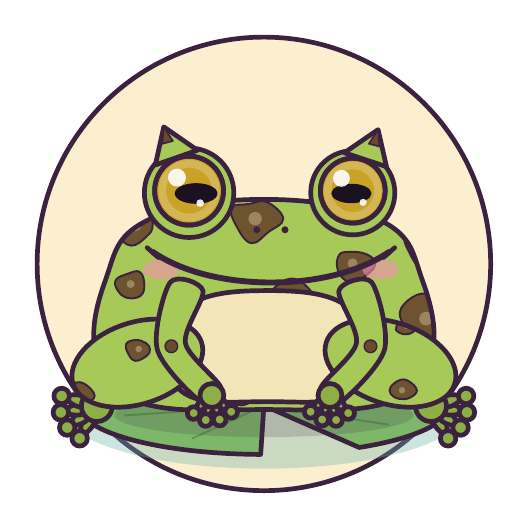
\begin{tikzpicture}
\clip (0,0) rectangle (6,6);
\filldraw[inked,fill=paper] (3,3) circle (2.88);
\fill[water, opacity=0.35] (3.0,1.15) ellipse (2.55 and 0.75);
\filldraw[inked,fill=pad] (3,1.2) -- ($(3,1.2)+(301:2.35 and 0.62)$) arc[start angle=301, end angle=629, x radius=2.35, y radius=0.62] -- cycle;
\draw[paddark, line width=0.7pt] (3,1.2) -- (4.587,0.958);
\draw[paddark, line width=0.7pt] (3,1.2) -- (4.771,1.325);
\draw[paddark, line width=0.7pt] (3,1.2) -- (3.916,1.619);
\draw[paddark, line width=0.7pt] (3,1.2) -- (2.526,1.667);
\draw[paddark, line width=0.7pt] (3,1.2) -- (1.413,1.442);
\draw[paddark, line width=0.7pt] (3,1.2) -- (1.229,1.075);
\draw[paddark, line width=0.7pt] (3,1.2) -- (2.084,0.781);
\fill[padlight, opacity=0.6] (2.178,1.417) ellipse (0.517 and 0.099);
\fill[ink, opacity=0.18] (3.0,1.08) ellipse (1.9 and 0.28);
\begin{scope}[shift={(3,1.15)}, rotate=0, xscale=0.893, yscale=0.893]
\filldraw[inked,fill=chompfeet] (-2.376,0.05) .. controls (-2.401,-0.231) .. (-2.62,-0.409) .. controls (-2.595,-0.128) .. (-2.376,0.05) -- cycle;
\filldraw[inked,fill=chompfeet] (-2.62,-0.409) circle (0.11);
\filldraw[inked,fill=chompfeet] (-2.376,0.05) .. controls (-2.522,-0.192) .. (-2.797,-0.256) .. controls (-2.651,-0.014) .. (-2.376,0.05) -- cycle;
\filldraw[inked,fill=chompfeet] (-2.797,-0.256) circle (0.11);
\filldraw[inked,fill=chompfeet] (-2.376,0.05) .. controls (-2.613,-0.103) .. (-2.888,-0.04) .. controls (-2.651,0.113) .. (-2.376,0.05) -- cycle;
\filldraw[inked,fill=chompfeet] (-2.888,-0.04) circle (0.11);
\filldraw[inked,fill=chompfeet] (-2.376,0.05) .. controls (-2.656,0.016) .. (-2.876,0.193) .. controls (-2.596,0.227) .. (-2.376,0.05) -- cycle;
\filldraw[inked,fill=chompfeet] (-2.876,0.193) circle (0.11);
\filldraw[inked,fill=chompfeet] (-2.376,0.05) circle (0.22);
\filldraw[inked,fill=chompfeet] (2.376,0.05) .. controls (2.595,-0.128) .. (2.62,-0.409) .. controls (2.401,-0.231) .. (2.376,0.05) -- cycle;
\filldraw[inked,fill=chompfeet] (2.62,-0.409) circle (0.11);
\filldraw[inked,fill=chompfeet] (2.376,0.05) .. controls (2.651,-0.014) .. (2.797,-0.256) .. controls (2.522,-0.192) .. (2.376,0.05) -- cycle;
\filldraw[inked,fill=chompfeet] (2.797,-0.256) circle (0.11);
\filldraw[inked,fill=chompfeet] (2.376,0.05) .. controls (2.651,0.113) .. (2.888,-0.04) .. controls (2.613,-0.103) .. (2.376,0.05) -- cycle;
\filldraw[inked,fill=chompfeet] (2.888,-0.04) circle (0.11);
\filldraw[inked,fill=chompfeet] (2.376,0.05) .. controls (2.596,0.227) .. (2.876,0.193) .. controls (2.656,0.016) .. (2.376,0.05) -- cycle;
\filldraw[inked,fill=chompfeet] (2.876,0.193) circle (0.11);
\filldraw[inked,fill=chompfeet] (2.376,0.05) circle (0.22);
\fill[chompskin] plot[smooth cycle, tension=0.7] coordinates {(0,0) (1.74,0.094) (2.376,0.752) (2.256,1.833) (1.68,2.679) (0,2.989) (-1.68,2.679) (-2.256,1.833) (-2.376,0.752) (-1.74,0.094)};
\begin{scope}\clip plot[smooth cycle, tension=0.7] coordinates {(0,0) (1.74,0.094) (2.376,0.752) (2.256,1.833) (1.68,2.679) (0,2.989) (-1.68,2.679) (-2.256,1.833) (-2.376,0.752) (-1.74,0.094)};
\filldraw[inked,fill=chompmark,line width=0.7pt,fill opacity=0.92] plot[smooth cycle, tension=0.7] coordinates {(0.275,2.715) (0.041,2.952) (-0.213,2.923) (-0.461,2.872) (-0.394,2.616) (-0.184,2.367) (0.064,2.524)};
\fill[chompbelly, opacity=0.35] (-0.124,2.715) circle (0.095);
\filldraw[inked,fill=chompmark,line width=0.7pt,fill opacity=0.92] plot[smooth cycle, tension=0.7] coordinates {(0.72,1.499) (0.64,1.72) (0.361,1.86) (0.052,1.602) (0.154,1.353) (0.373,1.139) (0.668,1.261)};
\fill[chompbelly, opacity=0.35] (0.448,1.499) circle (0.097);
\filldraw[inked,fill=chompmark,line width=0.7pt,fill opacity=0.92] plot[smooth cycle, tension=0.7] coordinates {(-1.701,1.785) (-1.766,1.958) (-1.94,1.93) (-2.107,1.841) (-2.077,1.691) (-1.941,1.588) (-1.752,1.619)};
\fill[chompbelly, opacity=0.35] (-1.896,1.785) circle (0.057);
\filldraw[inked,fill=chompmark,line width=0.7pt,fill opacity=0.92] plot[smooth cycle, tension=0.7] coordinates {(-0.122,0.24) (-0.176,0.371) (-0.337,0.445) (-0.463,0.325) (-0.496,0.148) (-0.331,0.06) (-0.18,0.122)};
\fill[chompbelly, opacity=0.35] (-0.294,0.24) circle (0.056);
\filldraw[inked,fill=chompmark,line width=0.7pt,fill opacity=0.92] plot[smooth cycle, tension=0.7] coordinates {(-1.582,2.614) (-1.657,2.829) (-1.896,2.807) (-2.053,2.694) (-2.071,2.482) (-1.886,2.331) (-1.672,2.458)};
\fill[chompbelly, opacity=0.35] (-1.824,2.614) circle (0.079);
\filldraw[inked,fill=chompmark,line width=0.7pt,fill opacity=0.92] plot[smooth cycle, tension=0.7] coordinates {(1.714,0.605) (1.65,0.753) (1.465,0.861) (1.27,0.678) (1.284,0.492) (1.452,0.347) (1.704,0.419)};
\fill[chompbelly, opacity=0.35] (1.517,0.605) circle (0.07);
\filldraw[inked,fill=chompmark,line width=0.7pt,fill opacity=0.92] plot[smooth cycle, tension=0.7] coordinates {(1.792,2.897) (1.696,3.03) (1.526,3.098) (1.343,2.983) (1.367,2.824) (1.523,2.704) (1.697,2.757)};
\fill[chompbelly, opacity=0.35] (1.573,2.897) circle (0.061);
\filldraw[inked,fill=chompmark,line width=0.7pt,fill opacity=0.92] plot[smooth cycle, tension=0.7] coordinates {(1.585,2.08) (1.456,2.21) (1.215,2.243) (1.065,2.192) (1.055,1.972) (1.216,1.817) (1.46,1.912)};
\fill[chompbelly, opacity=0.35] (1.262,2.08) circle (0.071);
\filldraw[inked,fill=chompmark,line width=0.7pt,fill opacity=0.92] plot[smooth cycle, tension=0.7] coordinates {(2.696,1.293) (2.5,1.504) (2.244,1.648) (1.951,1.439) (2.002,1.181) (2.221,0.965) (2.56,1.114)};
\fill[chompbelly, opacity=0.35] (2.306,1.293) circle (0.097);
\filldraw[inked,fill=chompmark,line width=0.7pt,fill opacity=0.92] plot[smooth cycle, tension=0.7] coordinates {(-0.948,1.236) (-1.091,1.459) (-1.291,1.416) (-1.461,1.343) (-1.461,1.149) (-1.315,1.039) (-1.056,1.111)};
\fill[chompbelly, opacity=0.35] (-1.244,1.236) circle (0.072);
\filldraw[inked,fill=chompmark,line width=0.7pt,fill opacity=0.92] plot[smooth cycle, tension=0.7] coordinates {(2.706,2.36) (2.57,2.579) (2.242,2.682) (2.008,2.495) (2.062,2.244) (2.262,2.001) (2.597,2.067)};
\fill[chompbelly, opacity=0.35] (2.327,2.36) circle (0.097);
\filldraw[inked,fill=chompmark,line width=0.7pt,fill opacity=0.92] plot[smooth cycle, tension=0.7] coordinates {(-1.718,0.374) (-1.713,0.501) (-1.917,0.51) (-2.025,0.447) (-2.102,0.291) (-1.92,0.212) (-1.775,0.216)};
\fill[chompbelly, opacity=0.35] (-1.879,0.374) circle (0.059);
\end{scope}
\draw[inked] plot[smooth cycle, tension=0.7] coordinates {(0,0) (1.74,0.094) (2.376,0.752) (2.256,1.833) (1.68,2.679) (0,2.989) (-1.68,2.679) (-2.256,1.833) (-2.376,0.752) (-1.74,0.094)};
\fill[chompbelly] plot[smooth cycle, tension=0.7] coordinates {(0.05,0.113) (1.19,0.207) (1.43,0.846) (1.13,1.504) (0.05,1.692) (-1.03,1.504) (-1.33,0.846) (-1.09,0.207)};
\draw[inked] plot[smooth cycle, tension=0.7] coordinates {(0.05,0.113) (1.19,0.207) (1.43,0.846) (1.13,1.504) (0.05,1.692) (-1.03,1.504) (-1.33,0.846) (-1.09,0.207)};
\fill[chompskin] [rotate around={18:(-1.8,0.66)}] (-1.8,0.66) ellipse (0.96 and 0.58);
\begin{scope}\clip [rotate around={18:(-1.8,0.66)}] (-1.8,0.66) ellipse (0.96 and 0.58);
\filldraw[inked,fill=chompmark,line width=0.7pt,fill opacity=0.92] plot[smooth cycle, tension=0.7] coordinates {(-2.407,0.199) (-2.547,0.363) (-2.698,0.376) (-2.804,0.267) (-2.838,0.121) (-2.691,0.056) (-2.53,0.087)};
\fill[chompbelly, opacity=0.35] (-2.649,0.199) circle (0.054);
\filldraw[inked,fill=chompmark,line width=0.7pt,fill opacity=0.92] plot[smooth cycle, tension=0.7] coordinates {(-1.621,0.861) (-1.677,0.946) (-1.819,0.989) (-1.957,0.937) (-1.929,0.794) (-1.828,0.693) (-1.664,0.766)};
\fill[chompbelly, opacity=0.35] (-1.78,0.861) circle (0.047);
\end{scope}
\draw[inked] [rotate around={18:(-1.8,0.66)}] (-1.8,0.66) ellipse (0.96 and 0.58);
\fill[chompskin] [rotate around={-18:(1.8,0.66)}] (1.8,0.66) ellipse (0.96 and 0.58);
\begin{scope}\clip [rotate around={-18:(1.8,0.66)}] (1.8,0.66) ellipse (0.96 and 0.58);
\filldraw[inked,fill=chompmark,line width=0.7pt,fill opacity=0.92] plot[smooth cycle, tension=0.7] coordinates {(2.176,0.274) (2.059,0.404) (1.932,0.419) (1.802,0.319) (1.807,0.218) (1.925,0.152) (2.077,0.169)};
\fill[chompbelly, opacity=0.35] (1.964,0.274) circle (0.046);
\filldraw[inked,fill=chompmark,line width=0.7pt,fill opacity=0.92] plot[smooth cycle, tension=0.7] coordinates {(1.632,1.136) (1.55,1.25) (1.391,1.295) (1.321,1.186) (1.321,1.073) (1.393,1.015) (1.516,1.048)};
\fill[chompbelly, opacity=0.35] (1.428,1.136) circle (0.045);
\filldraw[inked,fill=chompmark,line width=0.7pt,fill opacity=0.92] plot[smooth cycle, tension=0.7] coordinates {(2.169,1.186) (2.106,1.279) (2,1.333) (1.924,1.237) (1.876,1.138) (1.993,1.071) (2.114,1.098)};
\fill[chompbelly, opacity=0.35] (2.023,1.186) circle (0.038);
\end{scope}
\draw[inked] [rotate around={-18:(1.8,0.66)}] (1.8,0.66) ellipse (0.96 and 0.58);
\filldraw[inked,fill=chompskin] plot[smooth cycle, tension=0.5] coordinates {(-0.867,1.691) (-1.116,0.946) (-0.609,0.308) (-0.871,0.092) (-1.516,0.854) (-1.333,1.809)};
\filldraw[inked,fill=chompmark,line width=0.5pt] (-1.316,0.9) circle (0.09);
\filldraw[inked,fill=chompfeet] (-0.74,0.2) .. controls (-0.551,0.146) .. (-0.464,-0.031) .. controls (-0.654,0.023) .. (-0.74,0.2) -- cycle;
\filldraw[inked,fill=chompfeet] (-0.464,-0.031) circle (0.09);
\filldraw[inked,fill=chompfeet] (-0.74,0.2) .. controls (-0.608,0.054) .. (-0.629,-0.142) .. controls (-0.76,0.004) .. (-0.74,0.2) -- cycle;
\filldraw[inked,fill=chompfeet] (-0.629,-0.142) circle (0.09);
\filldraw[inked,fill=chompfeet] (-0.74,0.2) .. controls (-0.706,0.006) .. (-0.827,-0.149) .. controls (-0.861,0.045) .. (-0.74,0.2) -- cycle;
\filldraw[inked,fill=chompfeet] (-0.827,-0.149) circle (0.09);
\filldraw[inked,fill=chompfeet] (-0.74,0.2) .. controls (-0.814,0.017) .. (-0.999,-0.05) .. controls (-0.925,0.133) .. (-0.74,0.2) -- cycle;
\filldraw[inked,fill=chompfeet] (-0.999,-0.05) circle (0.09);
\filldraw[inked,fill=chompfeet] (-0.74,0.2) circle (0.17);
\filldraw[inked,fill=chompskin] plot[smooth cycle, tension=0.5] coordinates {(1.533,1.809) (1.716,0.854) (1.071,0.092) (0.809,0.308) (1.316,0.946) (1.067,1.691)};
\filldraw[inked,fill=chompmark,line width=0.5pt] (1.516,0.9) circle (0.09);
\filldraw[inked,fill=chompfeet] (0.94,0.2) .. controls (0.854,0.023) .. (0.664,-0.031) .. controls (0.751,0.146) .. (0.94,0.2) -- cycle;
\filldraw[inked,fill=chompfeet] (0.664,-0.031) circle (0.09);
\filldraw[inked,fill=chompfeet] (0.94,0.2) .. controls (0.96,0.004) .. (0.829,-0.142) .. controls (0.808,0.054) .. (0.94,0.2) -- cycle;
\filldraw[inked,fill=chompfeet] (0.829,-0.142) circle (0.09);
\filldraw[inked,fill=chompfeet] (0.94,0.2) .. controls (1.061,0.045) .. (1.027,-0.149) .. controls (0.906,0.006) .. (0.94,0.2) -- cycle;
\filldraw[inked,fill=chompfeet] (1.027,-0.149) circle (0.09);
\filldraw[inked,fill=chompfeet] (0.94,0.2) .. controls (1.125,0.133) .. (1.199,-0.05) .. controls (1.014,0.017) .. (0.94,0.2) -- cycle;
\filldraw[inked,fill=chompfeet] (1.199,-0.05) circle (0.09);
\filldraw[inked,fill=chompfeet] (0.94,0.2) circle (0.17);
\fill[ink] (-0.1,2.557) circle (0.05);
\fill[blush, opacity=0.6] (-1.46,1.993) ellipse (0.26 and 0.14);
\fill[ink] (0.3,2.557) circle (0.05);
\fill[blush, opacity=0.6] (1.66,1.993) ellipse (0.26 and 0.14);
\draw[ink, line width=2.125pt, line cap=round] (-1.58,2.242) .. controls (-0.74,1.662) and (0.94,1.662) .. (1.78,2.242);
\draw[ink, line width=1.7pt, line cap=round] (-1.5,2.162) -- (-1.66,2.302);
\draw[ink, line width=1.7pt, line cap=round] (1.7,2.162) -- (1.86,2.302);
\filldraw[inked,fill=chompskin] (-1.064,3.083) circle (0.636);
\filldraw[inked,fill=chompskin] (-0.944,3.688) -- (-1.424,4.02) -- (-1.544,3.478) -- cycle;
\filldraw[inked,fill=chompmark,line width=0.6pt] (-1.294,3.82) -- (-1.424,4.02) -- (-1.444,3.78) -- cycle;
\filldraw[inked,fill=chompeye] (-1.064,3.113) circle (0.49);
\draw[white, opacity=0.22, line width=2.72pt] (-1.064,3.113) circle (0.382);
\fill[pupil] (-0.964,3.073) ellipse (0.304 and 0.147);
\fill[white, opacity=0.9] (-1.236,3.299) circle (0.127);
\fill[white, opacity=0.9] (-0.907,2.937) circle (0.054);
\draw[inked] (-1.064,3.113) circle (0.49);
\filldraw[inked,fill=chompskin] (1.264,3.083) circle (0.598);
\filldraw[inked,fill=chompskin] (1.144,3.652) -- (1.624,3.981) -- (1.744,3.454) -- cycle;
\filldraw[inked,fill=chompmark,line width=0.6pt] (1.494,3.781) -- (1.624,3.981) -- (1.644,3.741) -- cycle;
\filldraw[inked,fill=chompeye] (1.264,3.113) circle (0.461);
\draw[white, opacity=0.22, line width=2.72pt] (1.264,3.113) circle (0.359);
\fill[pupil] (1.244,3.073) ellipse (0.286 and 0.138);
\fill[white, opacity=0.9] (1.103,3.288) circle (0.12);
\fill[white, opacity=0.9] (1.411,2.947) circle (0.051);
\draw[inked] (1.264,3.113) circle (0.461);
\end{scope}
\end{tikzpicture}
\end{document}
